\documentclass[final]{beamer}

\usepackage[scale=1.24]{beamerposter} % Use the beamerposter package for laying out the poster

\usetheme{confposter} % Use the confposter theme supplied with this template

\setbeamercolor{block title}{fg=nblue,bg=white} % Colors of the block titles
\setbeamercolor{block body}{fg=black,bg=white} % Colors of the body of blocks
\setbeamercolor{block alerted title}{fg=white,bg=dblue!70} % Colors of the highlighted block titles
\setbeamercolor{block alerted body}{fg=black,bg=dblue!10} % Colors of the body of highlighted blocks
% Many more colors are available for use in beamerthemeconfposter.sty

\usepackage[skins]{tcolorbox}
% a "sub-block" (plain block-within-block (second-level header))
\newenvironment{subblock}[1]{
  \setbeamertemplate{block begin}
  {
    \setbeamercolor{block title}{fg=nblue!90} % @TODO defer to beamercolortheme
    \par\vskip\medskipamount
    \begin{beamercolorbox}[colsep*=0ex,dp={2ex}]{block title}
      \vskip-0.5cm
      \begin{tikzpicture}[remember picture]
        \node (titlenode) at (0, 0) {\usebeamerfont{block title}\normalsize\insertblocktitle};
        \tcbsetmacrotowidthofnode{\titlewidth}{titlenode}
        \tcbsetmacrotoheightofnode{\titleheight}{titlenode}
        \shade [inner color=nblue!25!black!25,outer color=white]
        (-\titlewidth/2,-\titleheight/2-0.1cm) rectangle ++({1.1*\titlewidth},-0.2cm);
      \end{tikzpicture}
    \end{beamercolorbox}
    {\parskip0pt\par}
    \ifbeamercolorempty[bg]{block title}
    {}
    {\ifbeamercolorempty[bg]{block body}{}{\nointerlineskip\vskip-0.5pt}}
    \usebeamerfont{block body}
    \vskip-0.5cm
    \begin{beamercolorbox}[colsep*=0ex,vmode]{block body}
      \justifying
    }
    \setbeamertemplate{block end}
    {
    \end{beamercolorbox}
    \vskip\smallskipamount
  }
  \begin{block}{{\normalsize #1}}
  }{\end{block}}

\newlength{\sepwid}
\newlength{\colonewid}
\newlength{\coltwowid}
\newlength{\colthreewid}
\setlength{\paperwidth}{48in} % A0 width: 46.8in
\setlength{\paperheight}{36in} % A0 height: 33.1in
\setlength{\sepwid}{0.024\paperwidth} % Separation width (white space) between columns
\setlength{\colonewid}{0.27\paperwidth} % Width of column one
\setlength{\coltwowid}{0.28\paperwidth} % Width of column two
\setlength{\colthreewid}{0.354\paperwidth} % Width of one column
\setlength{\topmargin}{-0.5in} % Reduce the top margin size
% -----------------------------------------------------------

\usepackage{graphicx}  % Required for including images
\usepackage{booktabs} % Top and bottom rules for tables
\usepackage{tikz}
\usetikzlibrary{
  arrows,
  calc,
  decorations.pathmorphing,
  decorations.pathreplacing,
  decorations.markings,
  fadings,
  positioning,
  shapes,
  arrows.meta
}
\usepgfmodule{oo}

\pgfdeclareradialshading{glow2}{\pgfpoint{0cm}{0cm}}{
  color(0mm)=(white);
  color(2mm)=(white);
  color(8mm)=(black);
  color(10mm)=(black)
}
\pgfdeclareradialshading{glow}{\pgfpoint{0cm}{0cm}}{
  color(0mm)=(white);
  color(5mm)=(white);
  color(9mm)=(black);
  color(10mm)=(black)
}

\begin{tikzfadingfrompicture}[name=glow fading]
  \shade [shading=glow] (0,0) circle (1);
\end{tikzfadingfrompicture}

\begin{tikzfadingfrompicture}[name=glow2 fading]
  \shade [shading=glow2] (0,0) circle (1);
\end{tikzfadingfrompicture}

\pgfdeclarelayer{tweezer}
\pgfsetlayers{tweezer,main}
\pgfooclass{tweezer}{
  \method tweezer() {
  }
  \method drawTweezer(#1,#2,#3) {
    \begin{pgfonlayer}{tweezer}
      \shade[shading=radial,path fading=glow fading,shift={(#1,#2)},rotate=90,yscale=1,
      fill opacity=0.9,inner color=#3]
      plot[draw,samples=200,domain=-1.5:1.5] function {sqrt(0.01 + x**2 / 5)}
      -- plot[draw,samples=200,domain=1.5:-1.5] function {-sqrt(0.01 + x**2 / 5)};
    \end{pgfonlayer}
  }
  \method drawAtom(#1,#2,#3,#4) {
    \fill [#4,path fading=glow2 fading] (#1,#2) circle (#3);
  }
  \method drawNaAtom(#1,#2,#3) {
    \pgfoothis.drawAtom(#1,#2,#3,orange);
  }
  \method drawCsAtom(#1,#2,#3) {
    \pgfoothis.drawAtom(#1,#2,#3,blue);
  }
  \method drawNaTweezer(#1,#2) {
    \pgfoothis.drawTweezer(#1,#2,orange!35!black!30);
  }
  \method drawCsTweezer(#1,#2) {
    \pgfoothis.drawTweezer(#1,#2,blue!30!black!30);
  }
  \method up(#1,#2) {
    \pgfoothis.drawCsTweezer(#1,#2);
    \pgfoothis.drawNaAtom(#1,#2+0.06,0.12);
    \pgfoothis.drawCsAtom(#1,#2-0.06,0.16);
  }
  \method down(#1,#2) {
    \pgfoothis.drawCsTweezer(#1,#2);
    \pgfoothis.drawCsAtom(#1,#2+0.06,0.16);
    \pgfoothis.drawNaAtom(#1,#2-0.06,0.12);
  }
  \method naTrap(#1,#2) {
    \pgfoothis.drawNaTweezer(#1,#2);
    \pgfoothis.drawNaAtom(#1,#2,0.12);
  }
  \method csTrap(#1,#2) {
    \pgfoothis.drawCsTweezer(#1,#2);
    \pgfoothis.drawCsAtom(#1,#2,0.16);
  }
}
\pgfoonew \mytweezer=new tweezer()

% ----------------------------------------------------------------------------------------
%	TITLE SECTION
% ----------------------------------------------------------------------------------------

\def\realtitle{Association of single ultracold molecules in optical tweezers}

\title{%
  \texorpdfstring{%
    \makebox[\linewidth]{%
      \makebox[0pt][l]{%
        \raisebox{\dimexpr-\height+0.5\baselineskip}[0pt][0pt]
        {
\includegraphics[height=3\baselineskip]{harvard}}% Left logo
      }\hfill
      \makebox[0pt]{\textcolor{dblue}{\realtitle}}%
      \hfill\makebox[0pt][r]{%
        \raisebox{\dimexpr-\height+0.5\baselineskip}[0pt][0pt]
        {
\includegraphics[height=3\baselineskip]{cua}}% Right logo
      }%
    }%
  }
  {\realtitle}} % Poster title

\author{Yichao Yu, Jonathan Hood, Lee R. Liu, Jessie T. Zhang, Yen-Wei Lin,
  Kenneth Wang, Rem\'y Vatr\'e, Till Rosenband, Kang-Kuen Ni}
\institute{Harvard-MIT Center for Ultracold Atoms\\
  Department of Chemistry and Chemical Biology and Department of Physics, Harvard University}

% ----------------------------------------------------------------------------------------

\begin{document}

\addtobeamertemplate{block end}{}{\vspace*{2ex}} % White space under blocks
\addtobeamertemplate{block alerted end}{}{\vspace*{2ex}} % White space under highlighted (alert) blocks

\setlength{\belowcaptionskip}{2ex} % White space under figures
\setlength\belowdisplayshortskip{2ex} % White space under equations

\begin{frame}[t] % The whole poster is enclosed in one beamer frame
  \begin{columns}[t]
    \begin{column}{\sepwid}\end{column} % Empty spacer column
    \begin{column}{\colonewid} % The first column
      \begin{block}{Ultracold Molecules}
        \begin{columns}[T]
          \begin{column}{0.57\colonewid}
            \vspace{3ex}
            \begin{itemize}
            \item NaCs has a large permanent electric dipole moment ($\mathbf{4.6}$ \textbf{Debye})
            \item Strong anisotropic dipole-dipole interactions
            \item Coupled internal degrees of freedom
              can be used to tune interactions and store information
            \end{itemize}
          \end{column}
          \begin{column}{0.42\colonewid}
            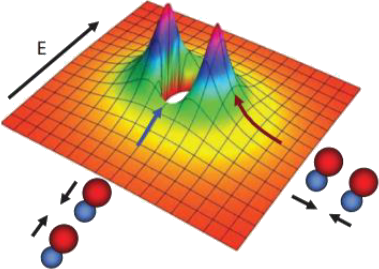
\includegraphics[width=0.4\colonewid]{reaction-align}
          \end{column}
        \end{columns}
        \begin{center}
          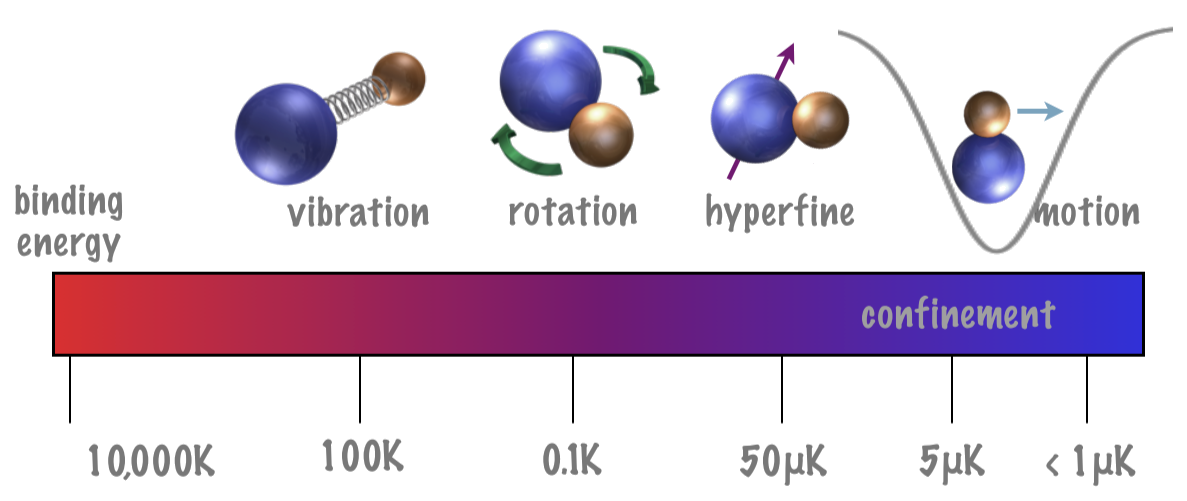
\includegraphics[width=0.8\colonewid]{temp-scale}
        \end{center}
      \end{block}

      \begin{block}{Our Approach}
        \begin{columns}[T]
          \begin{column}{0.6\colonewid}
            \vspace{1ex}
            \begin{itemize}
            \item Assemble and trap individual molecules in optical tweezers
              from laser-cooled atoms
            \item Raman transition from atoms to weakly-bound molecules
            \item STIRAP to ground state molecules
            \end{itemize}
            \vspace{2ex}
            \begin{subblock}{Advantages}
              \begin{itemize}
              \item Fast cycle time (<1s), small vacuum chamber
              \item Dynamically configurable trapping geometry
              \item All optical cooling and state-manipulation
              \end{itemize}
            \end{subblock}
            \vspace{2ex}
            \begin{subblock}{Quantum gate scheme}
              \begin{center}
                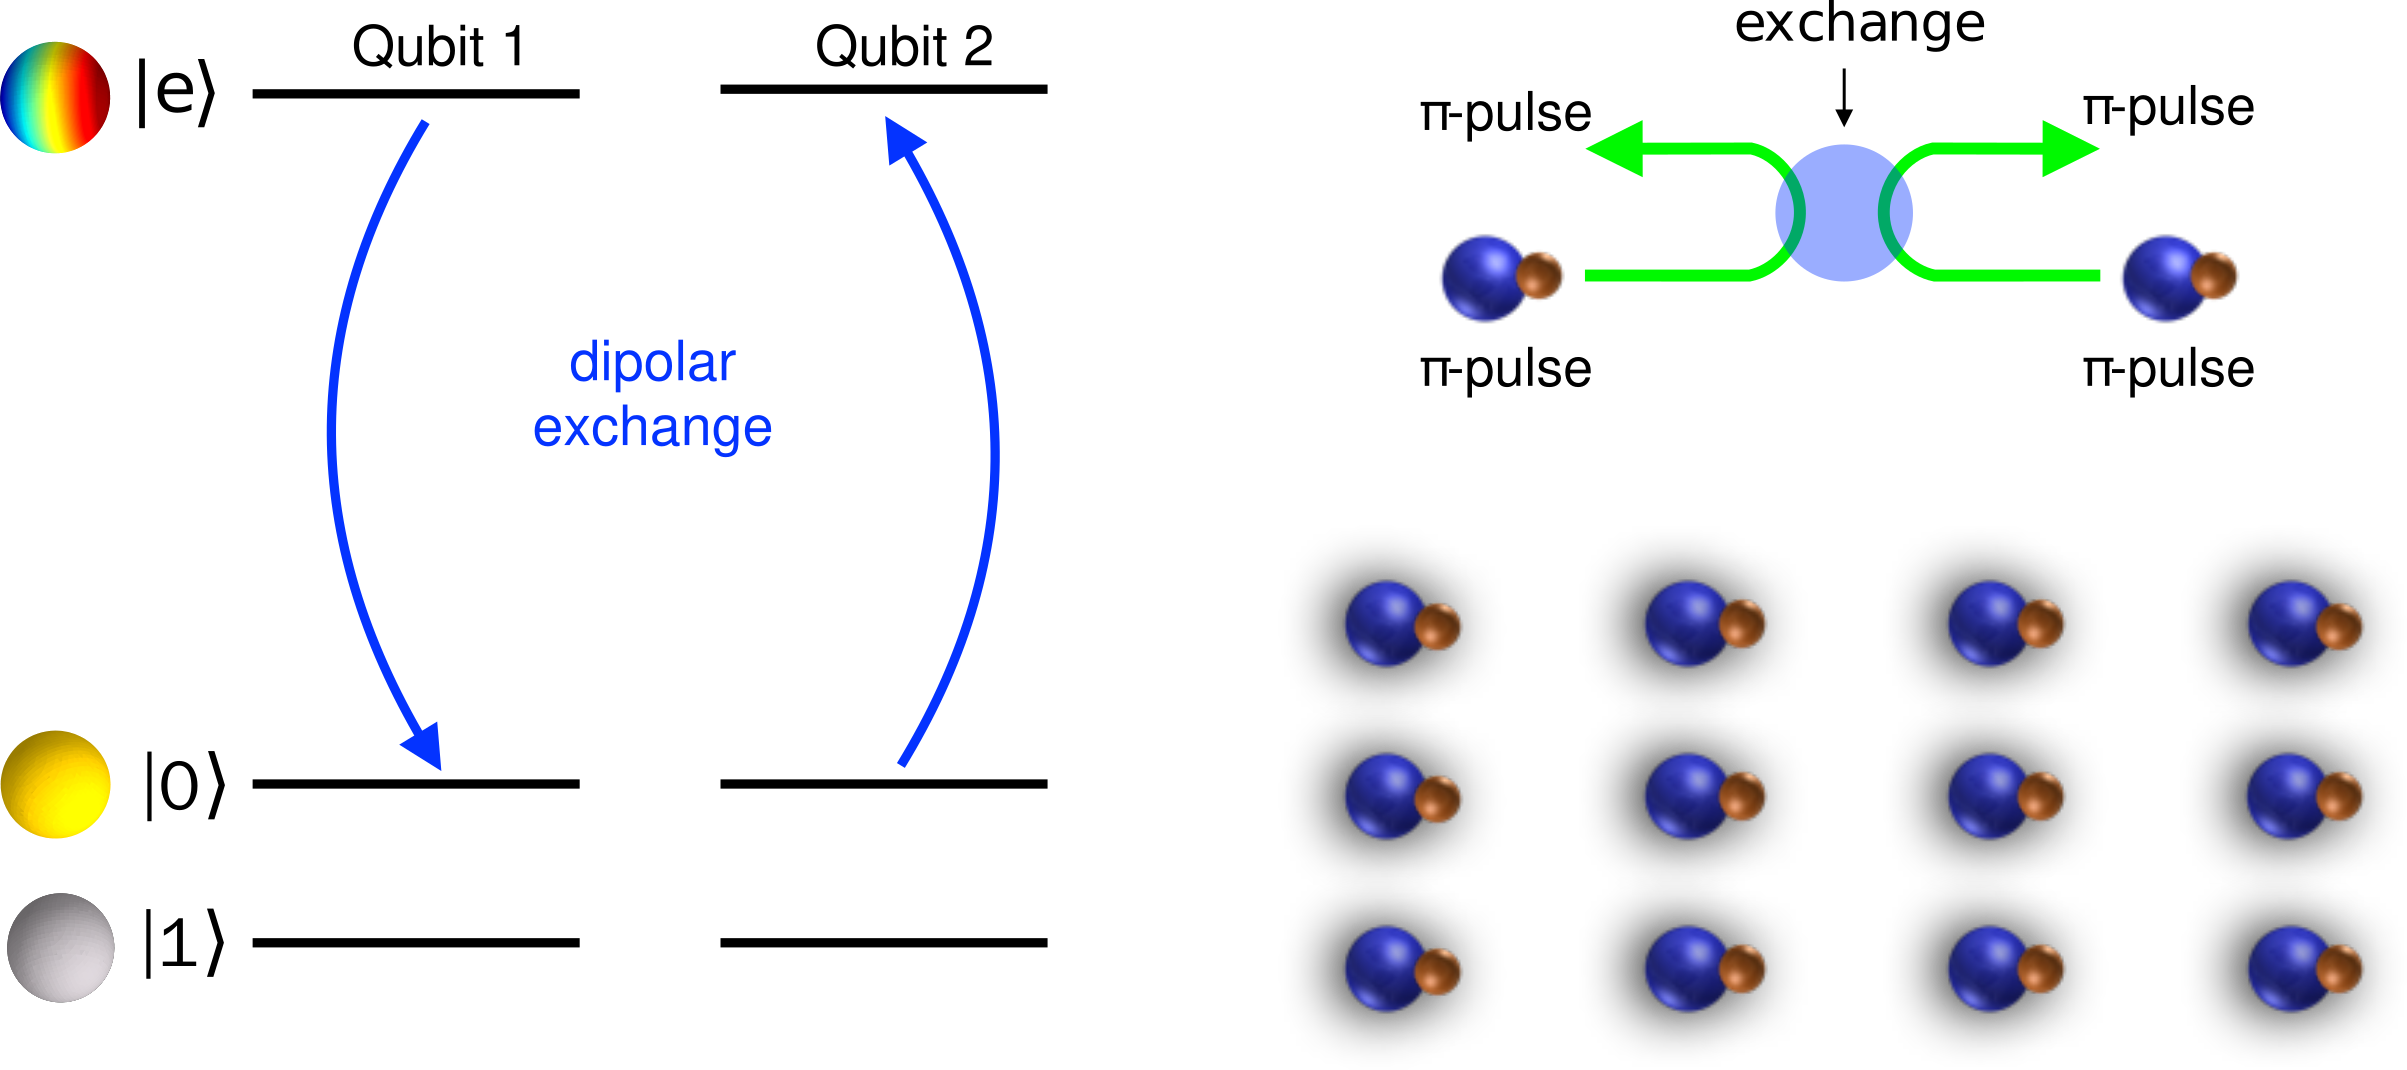
\includegraphics[width=0.6\colonewid]{quantum_gate}
              \end{center}
            \end{subblock}
          \end{column}
          \begin{column}{0.4\colonewid}
            \begin{tikzpicture}[scale=2.2]
              \foreach \xoff in {0,2.2} {
                \mytweezer.drawCsTweezer(0+\xoff, -0.5)
                \mytweezer.drawNaTweezer(-1+\xoff, -0.5)
                \mytweezer.drawCsAtom(-0.07+\xoff, -0.42, 0.22)
                \mytweezer.drawNaAtom(-1.06+\xoff, -0.59, 0.27)

                \mytweezer.drawCsTweezer(0+\xoff, -3.1)
                \mytweezer.drawNaTweezer(-1+\xoff, -3.1)
                \mytweezer.drawCsAtom(0.0+\xoff, -3.1, 0.12)
                \mytweezer.drawNaAtom(-1.0+\xoff, -3.1, 0.16)

                \mytweezer.drawCsTweezer(-1+\xoff, -7.0)
                \mytweezer.drawNaAtom(-1.05+\xoff, -6.87, 0.16)
                \mytweezer.drawCsAtom(-0.95+\xoff, -7.13, 0.12)

                \mytweezer.drawCsTweezer(-1+\xoff, -9.5)
                \mytweezer.drawNaAtom(-1.02+\xoff, -9.44, 0.16)
                \mytweezer.drawCsAtom(-0.98+\xoff, -9.56, 0.12)

                \begin{scope}[opacity=0.4]
                  \draw[orange,loosely dotted,line width=5] (-1+\xoff, -0.9) -- (-1+\xoff, -2.9);
                  \draw[blue,loosely dotted,line width=5] (0+\xoff, -0.65) -- (0+\xoff, -2.9);
                  \draw[-Latex,orange,line width=5] (-1+\xoff, -3.3) -- (-1+\xoff, -6.7);
                  \draw[-Latex,blue,domain=-3.3:-6.7,smooth,variable=\y,line width=5]
                  plot ({atan((\y+4.7) * 5) / 170 - 0.5+\xoff},{\y});
                \end{scope}
                \draw[orange!50!blue,loosely dotted,line width=5,opacity=0.7]
                (-1+\xoff, -7.3) -- (-1+\xoff, -9.3);
              }
              \node[below,rotate=-90] at (3.3, -1.8) {Trapping and cooling};
              \node[below,rotate=-90] at (2.3, -7) {Merging};
              \node[below,rotate=-90,align=center] at (2.9, -9.5) {Forming\\molecules};
            \end{tikzpicture}
          \end{column}
        \end{columns}
      \end{block}

      \begin{block}{Acknowledgements}
        \begin{center}
          
\includegraphics[height=0.18\colonewid]{beckman}
          \hspace{15ex}
\includegraphics[height=0.18\colonewid]{nsf}\\
          
\includegraphics[height=0.18\colonewid]{afosr}
          \hspace{5ex}
\includegraphics[height=0.18\colonewid]{sloan}
        \end{center}
      \end{block}
    \end{column} % End of the first column

    \begin{column}{\sepwid}\end{column} % Empty spacer column

    \begin{column}{\coltwowid}
      \begin{block}{Trapping and Cooling of Atoms}
        \begin{columns}[T]
          \begin{column}{0.45\coltwowid}
            \vspace{1ex}
            Laser-cooled and trapped single Cs and Na atoms < 100 uK in
            separate rearrangeable optical tweezers.\\
            \vspace{1ex}
            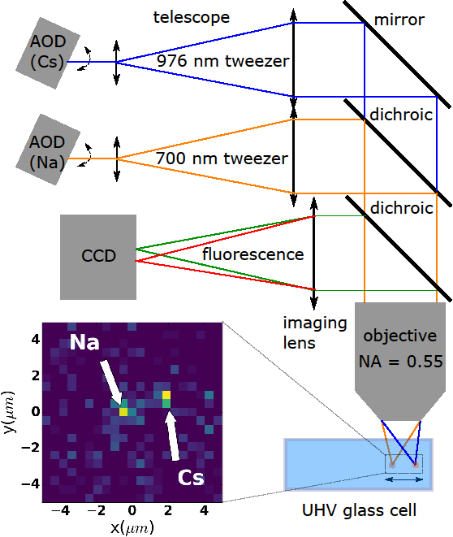
\includegraphics[width=0.45\coltwowid]{tweezer.png}
          \end{column}
          \begin{column}{0.55\coltwowid}
            \begin{tikzpicture}
              \node at (0, 0) {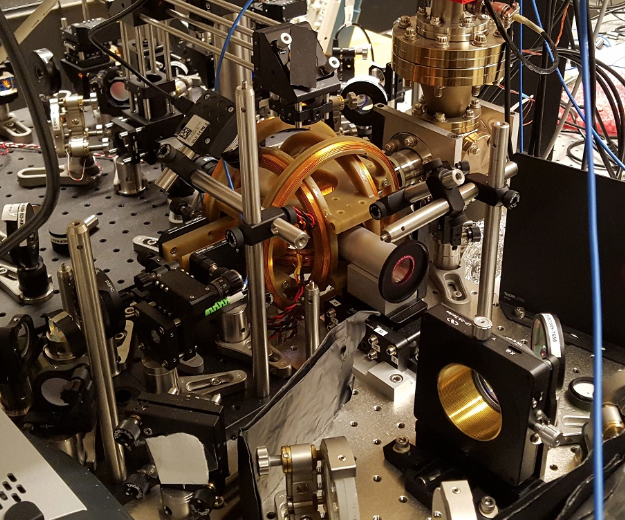
\includegraphics[width=0.46\coltwowid]{exp-photo}};
              \node[white,right,rotate=-27] at (0.5, 0.7) {\small \textbf{Tweezer}};
              \node[white,right,rotate=24] at (-0.46, 1.0) {\small \textbf{MOT}};
              \node[white,right,rotate=24] at (-0.54, 1.0) {\small \textbf{MOT}};
              \node[white,right,rotate=24] at (-0.5, 1.04) {\small \textbf{MOT}};
              \node[white,right,rotate=24] at (-0.5, 0.96) {\small \textbf{MOT}};
              \node[red!90!black,right,rotate=24] at (-0.5, 1) {\small \textbf{MOT}};
              \node[white,text width=0.2\coltwowid,align=center] at (-4.65, -1)
              {\baselineskip=0pt\small Single atom histogram};
              \node at (-4.65, -5.5) {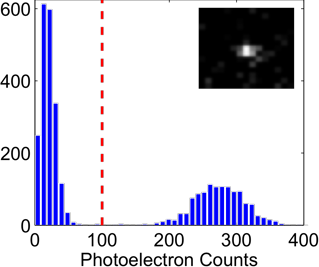
\includegraphics[width=0.24\coltwowid]{histogram}};
            \end{tikzpicture}
            \textit{\small Hutzler, Liu, Yu, Ni, New J. Phys 19, 023007 (2017)}\\
            \textit{\small L. Liu, Zhang, Yu, Hutzler, Hood, Liu, Rosenband, Ni,
              arXiv:1701.03121 (2017)}
          \end{column}
        \end{columns}
        \begin{columns}[T]
          \begin{column}{0.45\coltwowid}
            \vspace{1ex}
            \begin{center}
              \begin{tikzpicture}
                \node at (1, 10.9) {\textbf{Cs Raman spectrum}};
                \node at (0, 5.5) {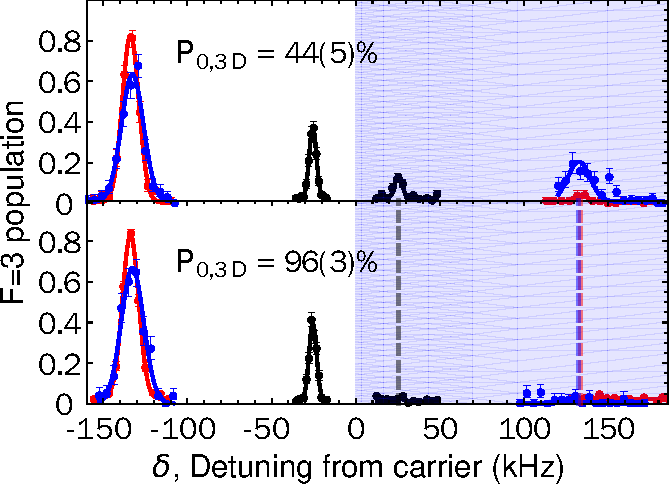
\includegraphics[width=0.4\coltwowid]{cs-raman}};
                \node at (1, -0.5) {\textbf{Na axial Raman spectrum}};
                \node at (0, -5.2) {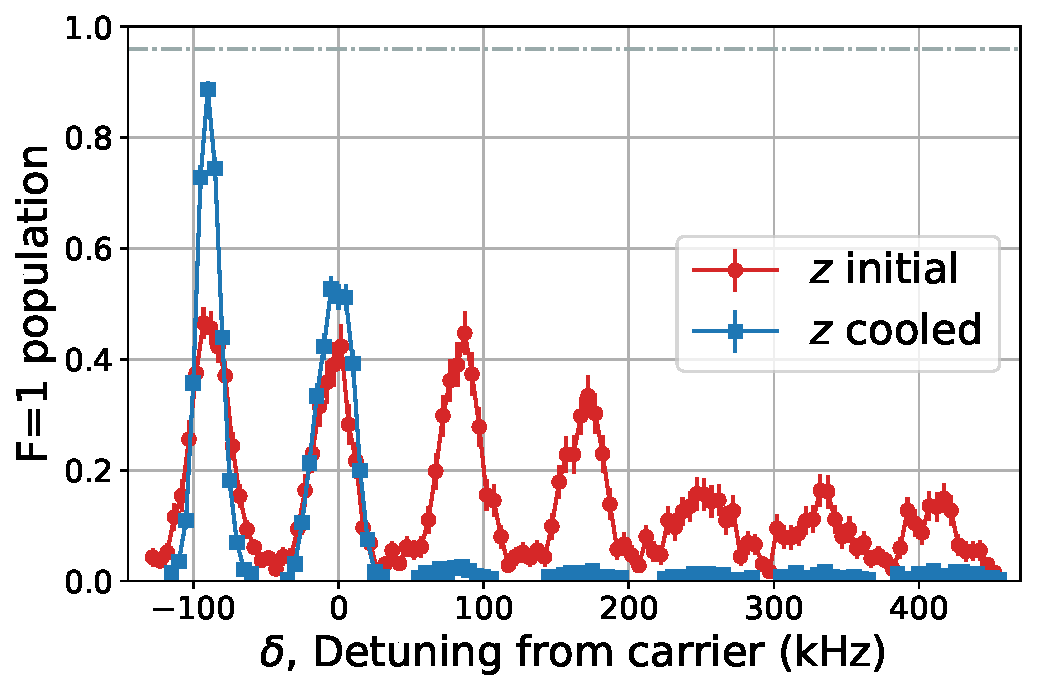
\includegraphics[width=0.4\coltwowid]{spectrum_nolabel_az}};
              \end{tikzpicture}
            \end{center}
          \end{column}
          \begin{column}{0.55\coltwowid}
            Cooled into motional ground states in the tweezers with Raman sideband cooling.
            Cooling fidelities are $96\%$ for Cesium and $94\%$ for Sodium.
            \vspace{2ex}
            \begin{center}
              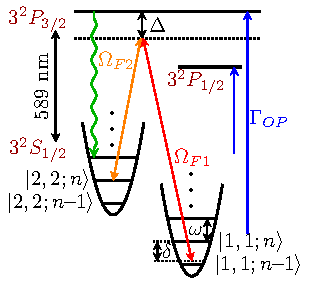
\includegraphics[width=0.47\coltwowid]{na-rsc-schematics}
            \end{center}
            {\small Yu, Hutzler, Zhang, L. Liu, Rosenband, Ni, arXiv:1708.03296 (2017)}
          \end{column}
        \end{columns}
      \end{block}
      \begin{block}{Merging Tweezers}
        \begin{itemize}
        \item Na and Cs tweezers are merged together into a single trap with little heating
        \item Observe hyperfine spin changing collisions when atoms in same trap
        \end{itemize}
        \begin{center}
          \begin{tikzpicture}
            \node[left] at (0, 0) {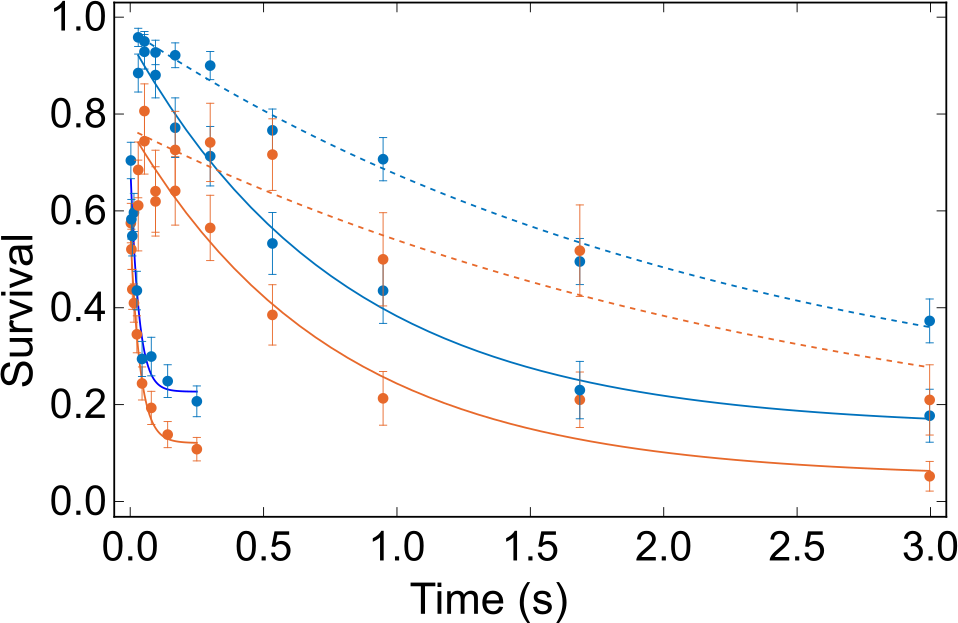
\includegraphics[width=0.7\coltwowid]{two-body-loss}};
            \mytweezer.drawCsAtom(2, 6.5, 0.8)
            \node[right,text width=0.25\coltwowid,align=left] at (0, 5) {Single body loss};
            \draw[{Latex}-,line width=5] (-9, 2) -- (0, 5.7);

            \draw[-{Latex},line width=5,blue!50!black] (2.1, 1.1) -- (1.9, -1.5);
            \mytweezer.drawCsAtom(2, 0, 0.8)
            \draw[-{Latex},line width=5,orange!50!black] (5.9, 1.1) -- (6.1, -1.5);
            \mytweezer.drawNaAtom(6, 0, 0.8)
            \node at (4, 0) {\large \textbf{+}};
            \node[right,text width=0.25\coltwowid,align=left] at (0.9, -2.3) {No spin flips};
            \draw[{Latex}-,line width=5] (-5, -2.3) -- (0.6, -2);


            \draw[{Latex}-,line width=5,blue!50!black] (-20.1, 1.5-9.5) -- (-19.9, -1.1-9.5);
            \mytweezer.drawCsAtom(-20, -9.5, 0.8)
            \draw[{Latex}-,line width=5,orange!50!black] (-15.9, 1.5-9.5) -- (-16.1, -1.1-9.5);
            \mytweezer.drawNaAtom(-16, -9.5, 0.8)
            \node at (-18, -9.5) {\large \textbf{+}};
            \draw[-{Latex},line width=6] (-14, -9.5) -- (-9, -9.5);
            \draw[-{Latex},line width=5,blue!50!black] (-7.1, 1.1-9.5) -- (-6.9, -1.5-9.5);
            \mytweezer.drawCsAtom(-7, -9.5, 0.8)
            \draw[-{Latex},line width=5,orange!50!black] (-2.9, 1.1-9.5) -- (-3.1, -1.5-9.5);
            \mytweezer.drawNaAtom(-3, -9.5, 0.8)
            \node at (-5, -9.5) {\large \textbf{+}};
            \node[right,text width=0.27\coltwowid,align=left] at (-1.5, -9.5)
            {Loss due to hyperfine state changing collision};
            \draw[{Latex}-,line width=5] (-19, -3) -- (-18.8, -7.7);
          \end{tikzpicture}
        \end{center}
      \end{block}
    \end{column} % End of the second column

    \begin{column}{\sepwid}\end{column} % Empty spacer column

    \begin{column}{\colthreewid} % The third column
      \begin{block}{Photoassociation}
        \begin{subblock}{Near threshold photoassociation}
          \begin{center}
            Simultaneous {\color{nblue}\textbf{Na}} and {\color{orange}\textbf{Cs}}
            loss due to photoassociation\\
            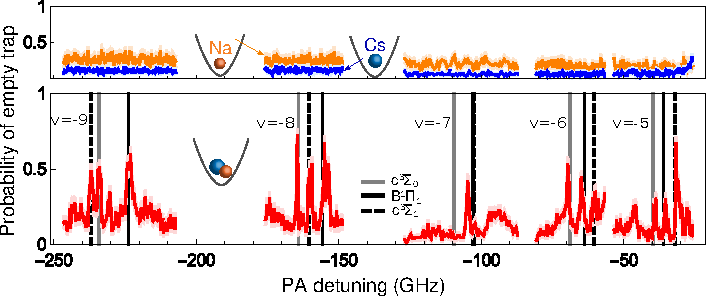
\includegraphics[width=0.85\colthreewid]{pa-shallow}\\
            PA Detuning from Cs D2 (GHz)
          \end{center}
        \end{subblock}
        \begin{columns}[T]
          \begin{column}{0.48\colthreewid}
            \begin{itemize}
            \item First photoassociation of a single molecule in an optical tweezer.
            \item Observation of new NaCs excited state vibrational lines near threshold.
            \item Vertical lines are fits to the LeRoy long range dispersion model,
              \[\Delta E\propto\frac{1}{\sqrt{C_6}}(v_D-v)^3\]
            \end{itemize}
            \vspace{1ex}
            \textit{\small Liu, Hood, Yu, Zhang, Hutzler Rosenband, Ni, Science 360, 6391 (2018)}
          \end{column}
          \begin{column}{0.48\colthreewid}
            \vspace{2ex}
            \begin{subblock}{Photoassociation for $v=0$ state}
              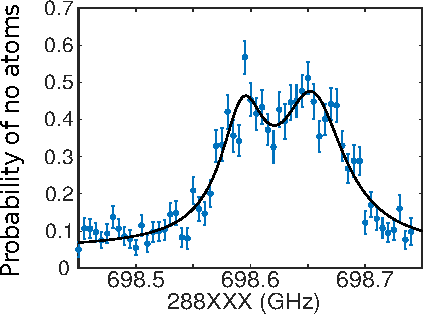
\includegraphics[width=0.4\colthreewid]{pa-v0}
            \end{subblock}
          \end{column}
        \end{columns}
      \end{block}

      \begin{block}{Coherent molecule formation \textit{\small (Preliminary)}}
        \begin{columns}[T]
          \begin{column}{0.44\colthreewid}
            \vspace{-1ex}
            \begin{center}
              \begin{tikzpicture}
                \begin{scope}
                  \draw[-Latex,line width=2.5] (0, 0) -- (0, 16);
                  \node[above,rotate=90] at (0, 8) {Energy};
                  \draw[-Latex,line width=2.5] (0, 0) -- (14, 0);
                  \node[below] at (7, 0) {Internuclear distance};

                  \draw[cyan!85!blue,line width=1.2] (2.0538 + 0.5, 3.5) -- (14, 3.5);
                  \draw[cyan!85!blue,line width=1.2] (2.1586 + 0.5, -0.9262 + 3.5) -- (9 + 0.5, -0.9262 + 3.5);
                  \draw[cyan!85!blue,Latex-Latex,line width=1.5] (7, 3.5) -- ++(0, -0.9262) node[midway, left]
                  {\small $\delta$};

                  \draw[line width=2.2,cyan!85!blue]
                  plot[samples=200,domain=1:6.75,variable=\x]
                  ({2*\x + 0.5}, {13.6*\x^(-3.4)-13.0*\x^(-1.7) + 3.5});
                  \node[cyan!85!blue] at (7.5, 0.9) {$a^3\Sigma^+$};

                  \draw[red,line width=1.2] (2.2204 - 1.5, -1.5440 + 15) -- (12 - 1.5, -1.5440 + 15);
                  \draw[red,line width=1.2] (2.7018 - 1.5, -3.5 + 15) -- (5.2197 - 1.5, -3.5 + 15);
                  \node[red,rotate=90] at (4 - 1.5, -2.5 + 15) {\textellipsis};

                  \draw[line width=2.2,red]
                  plot[samples=300,domain=1:7,variable=\x]
                  ({2*\x - 1.5}, {18.4*\x^(-2.5)-18.0*\x^(-1.3) + 15.0});
                  \node[above right,red] at (1.1, 14.4) {$c^3\Sigma^+$};

                  \mytweezer.drawNaAtom(13.1, 3.9, 0.4)
                  \mytweezer.drawCsAtom(14.1, 3.9, 0.35)

                  \mytweezer.drawNaAtom(8.16, 2.95, 0.4)
                  \mytweezer.drawCsAtom(8.5, 2.9, 0.35)

                  \draw[-Latex,green!70!black,line width=2] (13.6, 4.2) -- (8 - 1.5, -6 + 15);
                  \draw[Latex-,green!70!black,line width=2] (8.33, 3.1) -- (7.9 - 1.5, -6 + 15);
                  \draw[dashed,green!70!black,line width=3] (1, -6 + 15) -- (9, -6 + 15);
                  \draw[Latex-Latex,green!70!black,line width=3]
                  (3.7 - 1.5, -6 + 15) -- (3.7 - 1.5, -3.5 + 15) node[midway, right] {$\Delta$};
                \end{scope}
              \end{tikzpicture}\\
              \vspace{2ex}
              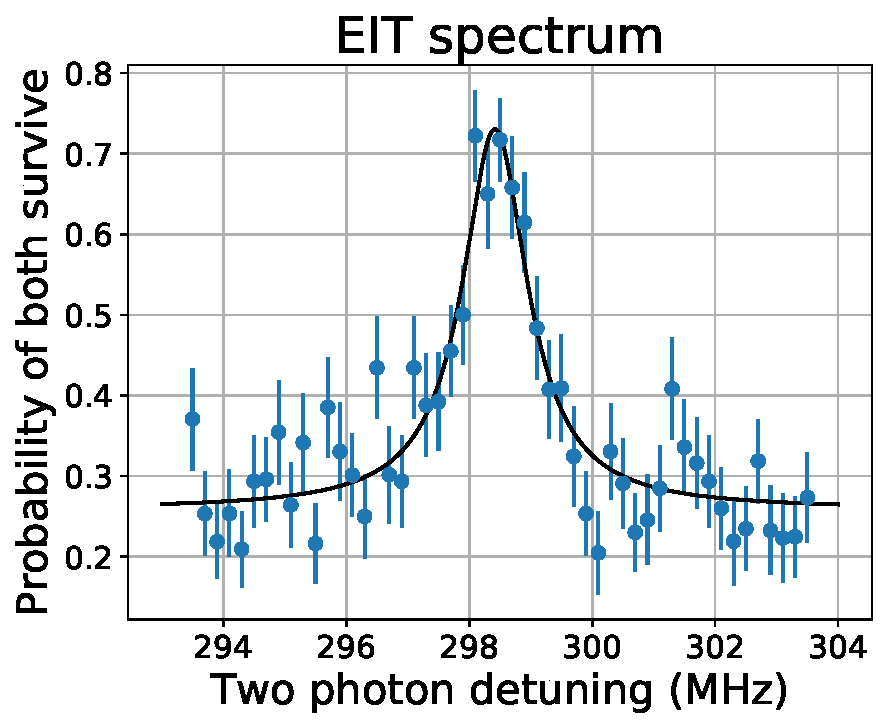
\includegraphics[width=0.42\colthreewid]{data_20180421_002556_eit-v0}
            \end{center}
          \end{column}
          \begin{column}{0.54\colthreewid}
            \begin{subblock}{Scheme}
              \begin{itemize}
              \item Raman transition to weakly-bound state
              \item STIRAP to rovibrational ground state
              \end{itemize}
            \end{subblock}
            \vspace{2ex}
            \begin{subblock}{Progress}
              \begin{itemize}
              \item Use electromagnetically induced transparency (EIT)
                to find the weakly-bound state.
                \[E_{\mathrm{binding}}=298.2\mathrm{MHz} \cdot h\]
              \item Observed Raman transition from atomic to molecular state
              \end{itemize}
            \end{subblock}
            \vspace{2ex}
            \begin{center}
              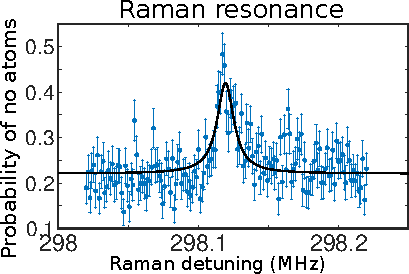
\includegraphics[width=0.48\colthreewid]{raman-v0}
            \end{center}
          \end{column}
        \end{columns}
      \end{block}

    \end{column} % End of the third column
  \end{columns} % End of all the columns in the poster

\end{frame} % End of the enclosing frame

\end{document}
